

\section{Дано}
   Проанализировать функцию 

\begin{equation}
    \centering
    \label{eq:eq1}
    y=\frac{5x}{4-x^2}
\end{equation}


\section{Решение}

\subsection{Область определения} 
    Ф-ция определена при x $\in \mathbb{R} \setminus\{-2; 2\}$
\subsection{Тип функции}\label{sec:2.2}
    Ф-ция не явяляется переодической.
    Проверим ф-цию на четность четность/нечетность:
   $ f(-x)=\frac{-5x}{4-x^2}  \Rightarrow (f(-x) \neq f(x)) \cap (f(-x) = -f(x)) \Rightarrow $ ф-ция является нечетной
\subsection{Рост функции}
    \[f’ = \frac{(5x)'(4-x^2)-5x(4-x^2)'}{(4-x^2)^2}
          = \frac{(5(4-x^2)-5x(-2x)}{(4-x^2)^2} 
          = \frac{20-5x^2+10x^2}{(4-x^2)^2} 
          = \frac{5(x^2+4)}{(4-x^2)^2}
     \]
    Таким образом, 
    \begin{equation}
    \centering
    \label{eq:eq2}
        f’ = \frac{5(x^2+4)}{(4-x^2)^2}
    \end{equation}

    График Данной функции будет выглядеть следющим образом \cite{matplotlib}
    \begin{figure}[H]
        \centering
        \includegraphics[height=10cm, width=15cm]{fig/firstDer.eps}
        \caption{График производной}
        \label{pic:derivative}
    \end{figure}
    Как видно из рис.~\ref{pic:derivative}, так и из самой функции производной можно с легкостью сделать вывод, что фунция возрастает на всей области определения
    
    

    
    
\subsection{Выпуклость функции}
    Возьмем вторую производную, чтобы узнать промежутки, в которых ф-ция выпукла вверх/вниз
    \begin{equation*}
        y'' = \frac{5((x^2+4)'(4-x^2)^2-(x^2+4)((4-x^2)^2)')}{(4-x^2)^4} =
        \frac{10x(x^2+12)}{4-x^2}
    \end{equation*}
    
    \begin{equation}
        \centering
        \label{eq:eq3}
        y'' =  \frac{10x(x^2+12)}{4-x^2}
    \end{equation}
    
    График данной функции будет выглядеть следющим образом \cite{matplotlib}
    \begin{figure}[H]
        \centering
        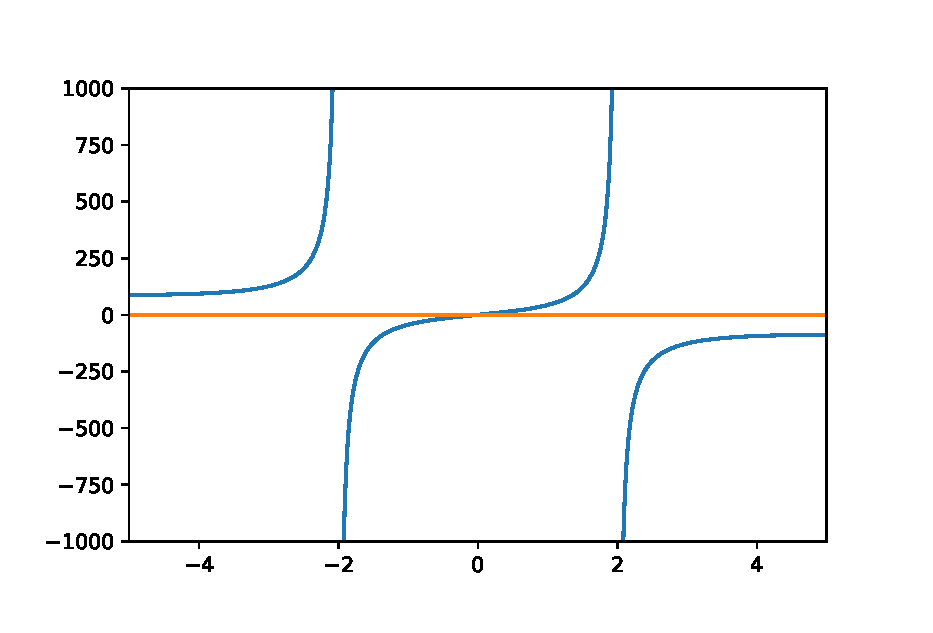
\includegraphics[width=\textwidth]{fig/secDer.eps} 
        \caption{График второй производной}
        \label{fig:my_label}
    \end{figure}
    Из этого можно сделать вывод, что ф-ция выпукла вверх при \\ $x \in (-\infty;-2)\cup(2;+\infty)$, а вниз во всех остальных точках определения ф-ции
    
\subsection{Нахождение асимптот}
    \subsubsection{Вертикальные асимптоты}
        Т.к. ф-ция не определена при $x = \pm2$, то целесообразно проверить эти точки на наличиеа асимптот:
        
        \noindent\begin{minipage}{.5\linewidth}
        \begin{equation}
            \label{eq:eq4}
            \lim_{x \to 2-0} \frac{5x}{4-x^2}=+\infty
        \end{equation}
        \end{minipage}%
        \begin{minipage}{.5\linewidth}
        \begin{equation}
            \label{eq:eq5}
            \lim_{x \to 2+0} \frac{5x}{4-x^2}=-\infty
        \end{equation}
        \end{minipage}
        
         Из $\eqref{eq:eq4}$ и  $\eqref{eq:eq5}$ следует, что $x = 2$ - вертикальная асимптота.\cite{zorichMath}
            
        \noindent\begin{minipage}{.5\linewidth}
        \begin{equation}
            \label{eq:eq6}
            \lim_{x \to -2-0} \frac{5x}{4-x^2}=+\infty
        \end{equation}
        \end{minipage}
        \begin{minipage}{.5\linewidth}
        \begin{equation}
            \label{eq:eq7}
            \lim_{x \to -2+0} \frac{5x}{4-x^2}=-\infty
        \end{equation}
        \end{minipage}
        \noindent Из $\eqref{eq:eq6}$ и  $\eqref{eq:eq7}$ следует, что $x = -2$ - вертикальная асимптота.
    \subsubsection{Горизонтальные асимптоты}
        Проверим существованиt(найдем) горизонатальные асимптоты:
        \begin{equation}
            \centering
            \label{eq:eq7}
            \lim_{x \to \infty} \frac{5x}{4-x^2}= \frac{5}{\infty} = 0
        \end{equation}
        \noindent Из $\eqref{eq:eq7}$ следует, что y=0 - горизонатальная асимптота
\subsection{Найдем точки пересечения ф-ции с координатными осями}
    \noindent\begin{minipage}{.5\linewidth}
        \begin{equation*}
            Ox:\frac{5x}{4-x^2}=0 \Rightarrow x=0
        \end{equation*}
        \end{minipage}%
        \begin{minipage}{.5\linewidth}
        \begin{equation*}
            Oy: y(0)=0 
        \end{equation*}
        \end{minipage}
\subsection{Найдем дополнительные точки}
	\begin{center}
		\begin{tabular}{|l|c|c|c|c|}
			\hline
			X & 1 & 1.5 & 3 & 5 \\ \hline
			Y & $\frac{5}{3}$ & $\frac{30}{7}$ & -3 & -$\frac{25}{21}$\\ \hline
		\end{tabular}
		\label{tabular:tab}
	\end{center}
	Нам этих точек хватит, так как ф-ция нечетная, что мы выяснили в секции \ref{sec:2.2}
	
\subsection{Начертим график}
    \begin{figure}[H]
        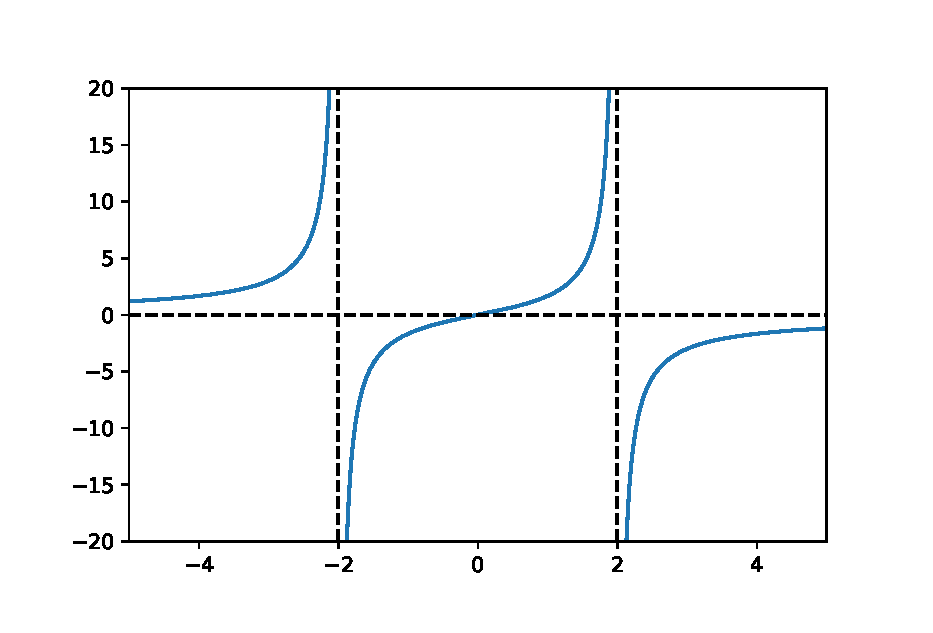
\includegraphics[width=\textwidth]{fig/mainPlot.eps} 
        \caption{график для $\eqref{eq:eq1}$}
        \label{fig:mainPlot}
    \end{figure}
    
\newpage
\section{Листинг}
    Это код, который был использован для создания рис. ~\ref{fig:mainPlot}
    \begin{code}
    	\inputminted[breaklines=true, xleftmargin=1em, linenos, frame=single, framesep=10pt, fontsize=\footnotesize, firstline=1, lastline=33]{python}{listings/python_code.py}
    	\caption{Питон - в массы)))}
    \end{code}

\newpage
\section*{Заключение}
В ходе проделанной типовой работы я смог проанализировать поведение ф-ции и построить её график, используя matplotlib
\addcontentsline{toc}{section}{Заключение}